\documentclass{beamer}
\usepackage[italian]{babel}
\usetheme{Berkeley}
\usepackage{graphicx}
\usepackage{booktabs}

\title{PineSU - Workflow}
\subtitle{Sviluppo di un'applicazione distribuita su Blockchain Ethereum}
\author{Paolo Speziali}
\institute{Università degli Studi di Perugia - Dipartimento di Ingegneria\\[\medskipamount]
      
\includegraphics[width=0.15\textwidth,height=0.15\textwidth]{figures/logo_unipg.png}%
 }
\logo{
\includegraphics[height=1cm]{figures/favicon.png}}
\date{A.A. 2020/2021}

\begin{document}
\begin{frame}
	\titlepage % beamer's \maketitle
\end{frame}
\section{Operazioni}
\begin{frame}
	\frametitle{Operazioni eseguibili}
	Nell'applicativo è possibile eseguire le seguenti operazioni:
	\begin{enumerate}
		\item Creazione di una Storage Unit (SU)
		\item Registrazione di una o più SU nella blockchain Ethereum
		\item Esportazione di sottoinsiemi di file da una SU
		\item Controllo d'integrità di singoli file esportati da altre SU
		\item Controllo d'integrità su una SU
	\end{enumerate}
	Oltre a poter eseguire tutti i comandi di Git. Vedremo ora questi comandi uno per uno utilizzando una directory campione da trasformare in Storage Unit.
\end{frame}
\begin{frame}
	\frametitle{Directory campione}
	Utilizzeremo come directory campione per mostrare l'evoluzione della Storage Unit una cartella chiamata \emph{sample} con la seguente struttura (dove \emph{first} e \emph{second} sono sottodirectory di \emph{sample} e \emph{third} è sottodirectory di \emph{second}):
	\smallskip
	\begin{figure}
		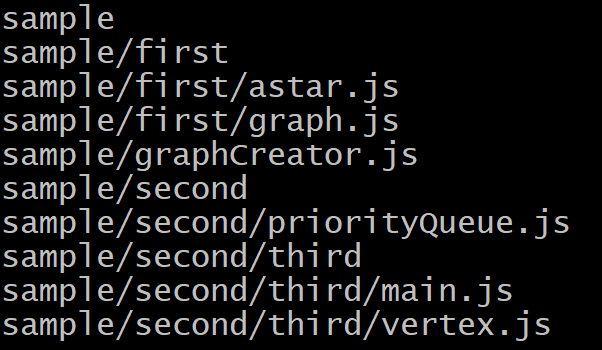
\includegraphics[width=0.80\textwidth]{figures/sample1.png}
	\end{figure}
\end{frame}
\section{Creazione}
\begin{frame}
	\frametitle{Creazione di una SU}
	La creazione di una Storage Unit è in realtà un'operazione che comprende sia la trasformazione in una Git Repository della directory, sia il calcolo degli hash che serviranno poi per registrare la nostra SU nella blockchain.
	\\

	Le informazioni della nostra SU sono conservate nel file \textbf{.pinesu.json} nella root della directory, la presenza di questo file indica al programma che la directory è già una SU.
	\\

	La creazione potrebbe eventualmente venire suddivisa in due azioni diverse, ma a quel punto la prima fase si limiterebbe ad eseguire un comando "git init" sulla directory, comando che potrebbe non essere necessario.
\end{frame}
\begin{frame}
	\frametitle{Creazione di una SU}
	Tuttavia, per come il programma è ora strutturato, la creazione della Storage Unit la rende pronta per essere registrata (eventualmente insieme ad altre) nella blockchain.
	\\

	Andiamo quindi a vedere quali sono le operazioni che avvengono in questa fase e come la nostra directory \emph{sample} cambia.
\end{frame}
\begin{frame}
	\frametitle{Creazione di una SU}
	\begin{itemize}
		\item Controlla se nella directory è già presente \textbf{.pinesu.json}, in caso negativo continua;
		\item Permette all'utente di selezionare dei file da ignorare da tutto il processo, ciò produce un file \textbf{.gitignore};
		\item Aggiunge tutti i file della directory nella Git Staging Area e crea un commit fantoccio;
		\item Recupera la lista dei file dal commit;
		\item Calcola gli hash di tutti i file (non directory);
		\item Calcola gli hash delle directory creando dei Merkle Tree (MT) con gli hash del loro contenuto e usa l'hash della radice come hash della directory, ciò avviene tramite un approccio bottom-up: calcola prima gli hash delle directory senza file al loro interno;
	\end{itemize}
\end{frame}
\begin{frame}
	\frametitle{Creazione di una SU}
	\begin{itemize}
		\item Calcola l'hash della SU creando un Merkle Tree con tutti gli hash dei file e delle directory in essa contenute e ne prende la radice;
		\item Viene generato il file \textbf{.pinesu.json} con al suo interno nome, descrizione, visibilità, data, hash dell'utente, hash della SU, lista dei file e delle sottodirectory con hash associati;
		\item Aggiunge tutti i file della directory nella Git Staging Area e crea un commit fantoccio;
		\item Aggiungo il percorso di questa SU con il suo hash alla lista della SU generate dall'utente (memorizzata nella cartella d'installazione del programma);
		\item Viene annullato il commit fantoccio e creato uno effettivo con informazioni consistenti e aggiunto \textbf{.pinesu.json};
	\end{itemize}
\end{frame}
\begin{frame}
	\frametitle{Creazione di una SU - Risultato}
	L'operazione di creazione ha prodotto nella cartella \emph{sample}, ovviamente, una sottocartella \emph{.git} e il file \textbf{.pinesu.json}. L'ordine di calcolo degli hash è stato questo:
	\newcounter{currentenumi}
	\begin{enumerate}
		\item sample/first/astar.js
		\item sample/first/graph.js
		\item sample/graphCreator.js
		\item sample/second/priorityQueue.js
		\item sample/second/third/main.js
		\item sample/second/third/vertex.js
		\setcounter{currentenumi}{\theenumi}
	\end{enumerate}
\end{frame}
\begin{frame}
	\frametitle{Creazione di una SU - Risultato}
	\begin{enumerate}
		\setcounter{enumi}{\thecurrentenumi}
		\item sample/first (tramite MT dei due file da lui contenuti)
		\item sample/second/third (tramite MT dei due file da lui contenuti)
		\item sample/second (tramite MT del file e della sottodirectory \emph{third} da lui contenuti)
		\item sample (tramite MT degli hash dei tutti i file e le directory appena visti)
	\end{enumerate}
	Si può quindi facilmente osservare come questa tecnica di calcolo di hash bottom-up viene messa in atto calcolando prima i file effettivi, poi le directory senza sottodirectory e infine tutto il resto delle directory.
	\end{frame}
\begin{frame}
	\frametitle{Chiarificazione}
	Mentre per le tre sottodirectory ci trovavamo in una situazione in cui il contenuto era composto da due soli elementi il Merkle Tree prodotto era ovviamente bilanciato, tuttavia per calcolare l'hash dell'intera directory \emph{sample} il MT prodotto aveva nove elementi, il nono elemento si trovava quindi scoppiato. La presenza di elementi in numero dispari è infatti l'unico motivo di sbilanciamento in questi MT in quanto, anziché essere l'albero a sistemare gli elementi in base alla struttura File System, andiamo a creare un albero per ogni directory ed esso si trova ad avere un numero \(n\) di elementi pronti da utilizzare. 
\end{frame}
\begin{frame}
	\frametitle{Chiarificazione}
	L'hash che verrà infine inserito nella blockchain non sarà tuttavia l'hash della directory \emph{sample}, bensì l'hash del suo file \textbf{.pinesu.json}, ogni volta quindi che farò riferimento all'hash della SU mi starò riferendo all'hash del file JSON associato.
\end{frame}
\section{Registrazione}
\begin{frame}
	\frametitle{Registrazione di una o più SU nella blockchain}
	In questa fase all'utente viene data la libertà di scegliere se registrare con un unico hash una o più SU insieme, poiché il workflow è praticamente identico andrò a separare i punti esclusivi ad una registrazione “multipla” scrivendoli in color oliva:
	\begin{itemize}
		\item Mostra la selezione multipla della SU registrate dall'utente per permettere di registrarne una sola o più in una volta;
		\item \textcolor{olive}{Per ogni Storage Unit selezionata} creo nella root della SU il file \textbf{.registration.json} che contiene l'hash della directory, l'hash che verrà salvato nella blockchain (stesso valore se registriamo una sola SU, \textcolor{olive}{valore della root del MT di tutti gli hash delle SU selezionate se la registrazione è multipla})
	\end{itemize}
\end{frame}
\begin{frame}
	\frametitle{Registrazione di una o più SU nella blockchain}
	\begin{itemize}
		\item \textcolor{olive}{Nel caso di una registrazione multipla, va a calcolare ed inserire in \textbf{.registration.json} le \emph{proof}, ovvero le informazioni che permettono di risalire all'hash registrato su blockchain dato l'hash della singola SU};
		\item Apre una scheda del browser per permettere il pagamento in ETH, nella blockchain sarà registrato l'hash della SU (\textcolor{olive}{o risultante da più SU}) unito all'hash personale dell'utente della registrazione (non si esclude infatti la possibilità di implementare un'autenticazione centralizzata).
	\end{itemize}
\end{frame}
\section{Esportazione}
\begin{frame}
	\frametitle{Esportazione di sottoinsiemi di file da una SU}
	In questa fase all'utente viene data la possibilità di scegliere di esportare alcuni file dalla SU, essi potranno poi in seguito essere integrati in altre SU e ne potrà essere controllata l'integrità:
	\begin{itemize}
		\item Mostra la selezione multipla dei file della SU per permettere all'utente di scegliere quali esportare;
		\item Viene creato un file \textbf{.pifiles.json} in cui salva, per ogni file esportato, il suo percorso originale, il suo hash, l'hash della root e le \emph{proof} per calcolare la root dato l'hash del file (ciò servirà nell'operazione di verifica d'integrità);
		\item I file, seguendo la struttura in cui comparivano nella SU originale, e \textbf{.pifiles.json} vengono compressi in un file ZIP (chiamato \textbf{pinesuExport.zip}) e salvati nella cartella precedente a quella in cui si sta operando;
	\end{itemize}
\end{frame}
\begin{frame}
	\frametitle{Esportazione di sottoinsiemi di file da una SU - Risultato}
	L'operazione di esportazione dei file \emph{sample/graphCreator.js}, \emph{sample/first/graph.js} e \emph{sample/second/third/main.js} ha prodotto un file \textbf{pinesuExport.zip} contenente i file esportati e la struttura delle cartelle mantenuta inalterata (\textcolor{red}{è presente un bug che taglia i nomi delle cartelle nel file ZIP, nulla di grave ma sto comunque investigando sulla causa di ciò}) e il file \textbf{.pifiles.json}.
\end{frame}
\section{Controllo file esportati}
\begin{frame}
	\frametitle{Controllo d'integrità di singoli file esportati da altre SU}
	L'unica operazione svolta dal controllo d'integrità dei file esportati è quella di cercare i \textbf{.pifiles.json} nella cartella d'interesse e controllare che l'hash di ogni file combaci con quello registrato nel documento JSON e che si riesca a risalire all'hash della SU originale tramite le \emph{proof} memorizzate sempre nel medesimo JSON. 
\end{frame}
\section{Controllo d'integrità su una SU}
\begin{frame}
	\frametitle{Controllo d'integrità su una SU}
	In questa operazione l'applicativo svolge un controllo d'integrità ricalcolando gli hash, confrontandoli con i dati registrati in precedenza e contollando la presenza dell'hash su blockchain.
	\begin{itemize}
		\item Avviene un ricalcolo degli hash di file e directory come descritto nella fase di creazione;
		\item Si legge il file \textbf{.pinesu.json} e si confrontano i dati appena calcolati con quelli vecchi;
		\item Si richiama l'operazione di controllo dei file integrati da altre SU;
		\item In caso i dati in \textbf{.pinesu.json} combacino con i dati appena calcolati si procede a controllare la presenza dell'hash della SU su blockchain, ciò avviene leggendo \textbf{.registration.json}, \textcolor{olive}{verificando le \emph{proof} del MT in caso di regsitrazione multipla} e cercando nella blockchain i dati richiesti.
	\end{itemize}
\end{frame}
\section{Workflow}
\begin{frame}
	\frametitle{Workflow di una Storage Unit}
	Nell'immagine della slide successiva è possibile osservare il riassunto, in forma grafica, dei concetti delle slide precedenti.
	I sensi delle frecce permettono di capire quali azioni cambiano lo stato di una Storage Unit e quali azioni sono irreversibili (almeno all'interno dell'applicativo).
\end{frame}
\begin{frame}
	\frametitle{Workflow di una Storage Unit}
	\begin{figure}
		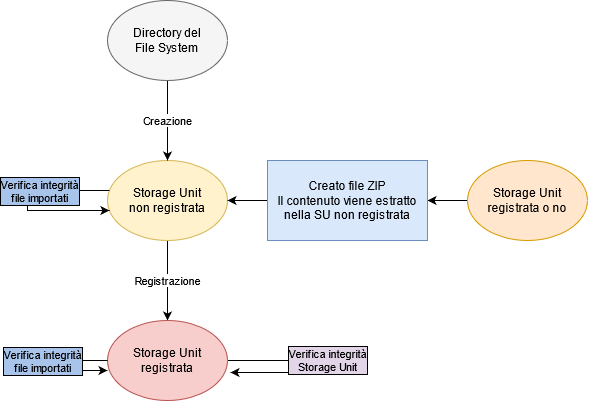
\includegraphics[width=\textwidth]{figures/WorkflowSU.png}
	\end{figure}
\end{frame}

\section{Resoconto}
\begin{frame}
	\frametitle{Resoconto}
	\begin{itemize}
  		\item Professore Tutor: Luca Grilli
  		\item Studente Tirocinante: Paolo Speziali
  		\item Anno Accademico: 2020/2021
	\end{itemize}
\end{frame}
\end{document}